\documentclass[tikz]{standalone}
\usepackage{tikz}
\usetikzlibrary{positioning,matrix,backgrounds}

\pgfdeclarelayer{background}
\pgfdeclarelayer{foreground}
\pgfsetlayers{background,main,foreground}

\begin{document}
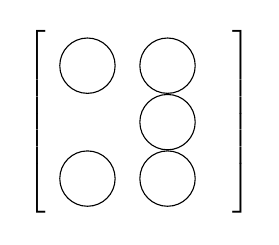
\begin{tikzpicture}

\matrix[matrix of nodes,column sep=3mm, left delimiter={[}, right delimiter={]}] (m)
{
 \draw(0,0) circle(10pt); & \draw(0,0) circle(10pt); &  \\
   & \draw(0,0) circle(10pt); &  \\
  \draw(0,0) circle(10pt); & \draw(0,0) circle(10pt); & \\
};

% \begin{pgfonlayer}{background}
% \foreach \i in {1,2,3}
%   \foreach \j in {1,2,3}
%     \node[draw, thick, red, circle] at (m-\i-\j) {Top};
% \end{pgfonlayer}

\end{tikzpicture}
\end{document}